\section{Results}
\label{sec:results}

We first compare each edit family against the noise floor (\secref{sec:res_overall}). We then break results down by edit (\secref{sec:res_cond}), model and size (\secref{sec:res_size}) and task (\secref{sec:res_task}), and we close with mediators of the effect (\secref{sec:res_mediators}).

\subsection{Invisible edits change outputs far above the noise floor}
\label{sec:res_overall}

\Tabref{tab:overall} shows the main result.
Re-running the byte-identical prompt flips 0.02\% of classification labels.
A single invisible edit flips 4.88\% \ci{4.61}{5.14}, more than 200 times the floor.
Perturbation \versus control is significant after Holm correction in 80 of 110 model $\times$ condition cells for label flips, 64 of 110 for code pass/fail flips and 89 of 110 for code text changes.
Most non-significant cells are \cond{ellipsis_char}, which touches few items, or punctuation edits on large models.

{\bf Is whitespace or punctuation more disruptive?}
We hypothesized that punctuation edits would cause more divergence (8--20\%) than whitespace edits (3--8\%).
The data show the reverse.
Whitespace edits flip 7.07\% of labels and punctuation edits 2.17\%, a difference of 4.9\pp \ci{4.6}{5.2}.
The same ordering holds for code text changes (47.6\% \versus 22.6\%) and code pass/fail flips (7.17\% \versus 2.79\%).
In a GEE model clustered by item, the odds ratio for punctuation relative to whitespace is 0.28 for label flips ($p<10^{-190}$) and 0.37 for code pass/fail flips.

\begin{table}[t]
    \centering
    \small
    \begin{tabular}{@{}llcccc@{}}
        \toprule
        \textbf{Task kind} & \textbf{Metric} & \textbf{Control} & \textbf{Whitespace} & \textbf{Punctuation} & \textbf{All edits} \\
        \midrule
        Classification & label flip & 0.02 & {\bf 7.07} & 2.17 & 4.88 \ci{4.61}{5.14} \\
        (1,200 items) & raw text changed & 0.13 & {\bf 11.7} & 5.2 & -- \\
        \midrule
        Code & code changed & 6.2 & {\bf 47.6} & 22.6 & 35.7 \ci{34.2}{37.4} \\
        (464 problems) & pass/fail flip & 0.61 & {\bf 7.17} & 2.79 & 5.08 \ci{4.69}{5.51} \\
        \bottomrule
    \end{tabular}
    \caption{Divergence from the canonical output (\%), averaged over items, models and conditions, with bootstrap 95\% CIs over items. Every edit family is far above the identical-prompt control, and whitespace (bold) exceeds punctuation on every metric. For classification flips, the punctuation $-$ whitespace difference is $-4.9$\pp \ci{$-5.2$}{$-4.6$}.}
    \label{tab:overall}
\end{table}


\subsection{Per-edit results}
\label{sec:res_cond}

\begin{figure}[t]
    \centering
    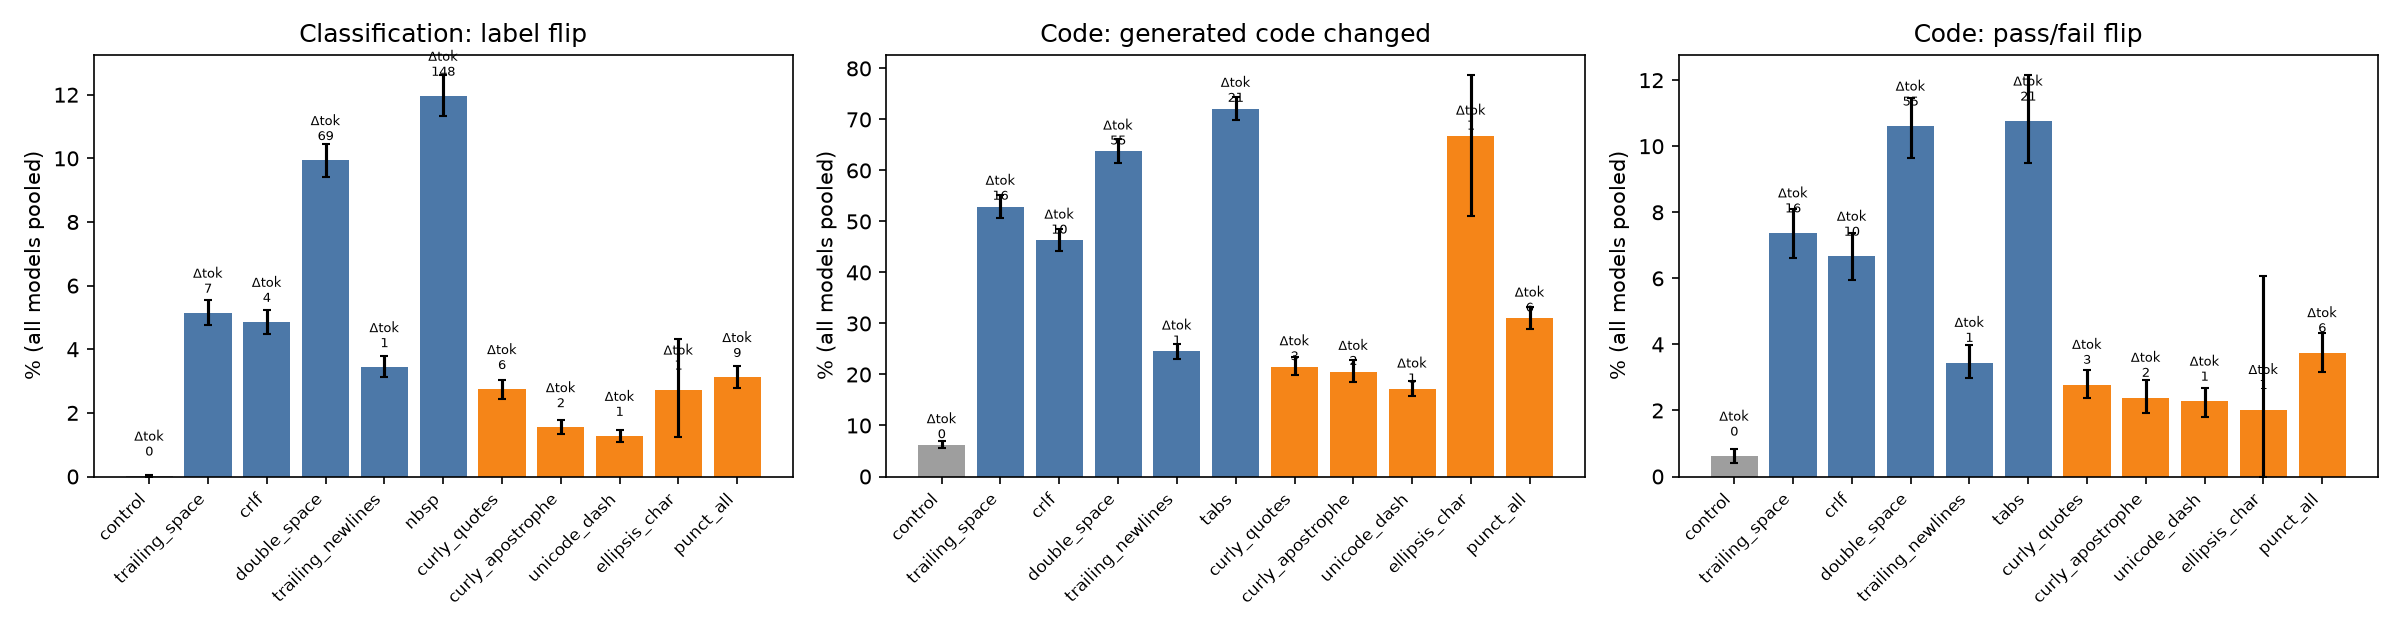
\includegraphics[width=0.99\linewidth]{figures/per_condition.png}
    \caption{Divergence per edit, pooled over 11 models, with bootstrap 95\% CIs. \figleft classification label flips. \figcenter code text changes. \figright code pass/fail flips. Blue bars are whitespace edits, orange bars punctuation edits, and grey is the identical-prompt control. Labels above the bars give \dtok, the mean number of changed prompt tokens. Every whitespace edit except \cond{trailing_newlines} exceeds every punctuation edit on label and pass/fail flips.}
    \label{fig:per_condition}
\end{figure}

\Figref{fig:per_condition} and \tabref{tab:per_condition} break the effect down by edit.
The two global whitespace edits are the most disruptive. \cond{nbsp} flips 12.0\% of labels and \cond{double_space} 9.9\%, and both rewrite dozens of tokens (\dtok of 148 and 69).
Yet even the local whitespace edits, which change only a few tokens, beat every single punctuation edit: \cond{trailing_space} flips 5.1\% and \cond{crlf} 4.9\%, against 1.3--2.7\% for the punctuation edits.
Combining all four punctuation edits (\cond{punct_all}, 3.1\%) is still less disruptive than any whitespace edit except \cond{trailing_newlines}.
On code, \cond{tabs} changes 72.1\% of generations and flips 10.8\% of pass/fail outcomes.
Indentation and line-end characters in the prompt propagate into how the model formats its own code.

\begin{table}[t]
    \centering
    \small
    \begin{tabular}{@{}llccccc@{}}
        \toprule
        & & \multicolumn{2}{c}{\textbf{Classification}} & \multicolumn{3}{c}{\textbf{Code}} \\
        \cmidrule(lr){3-4} \cmidrule(lr){5-7}
        \textbf{Family} & \textbf{Condition} & \dtok & label flip & \dtok & code changed & pass/fail flip \\
        \midrule
        Control & \ctrl & 0 & 0.02 & 0 & 6.2 & 0.6 \\
        \midrule
        \multirow{5}{*}{Whitespace} & \cond{trailing_space} & 7.4 & 5.1 & 16.3 & 52.9 & 7.4 \\
        & \cond{crlf} & 4.3 & 4.9 & 10.1 & 46.3 & 6.7 \\
        & \cond{double_space} & 68.9 & 9.9 & 54.5 & 63.7 & 10.6 \\
        & \cond{trailing_newlines} & 0.7 & 3.4 & 1.5 & 24.5 & 3.5 \\
        & \cond{nbsp} / \cond{tabs} & 147.7 & {\bf 12.0} & 20.8 & {\bf 72.1} & {\bf 10.8} \\
        \midrule
        \multirow{5}{*}{Punctuation} & \cond{curly_quotes} & 6.1 & 2.7 & 3.2 & 21.5 & 2.8 \\
        & \cond{curly_apostrophe} & 1.8 & 1.5 & 2.1 & 20.6 & 2.4 \\
        & \cond{unicode_dash} & 1.3 & 1.3 & 1.1 & 17.1 & 2.3 \\
        & \cond{ellipsis_char}$^*$ & 1.2 & 2.7 & 1.4 & 66.7 & 2.0 \\
        & \cond{punct_all} & 9.2 & 3.1 & 6.3 & 31.0 & 3.7 \\
        \bottomrule
    \end{tabular}
    \caption{Divergence (\%) per edit, pooled over 11 models. \dtok is the mean number of prompt token positions changed after the chat template and tokenizer. The most disruptive edit in each column is in bold. $^*$\cond{ellipsis_char} applies to only 40 classification and 9 code items per model, so its CIs are very wide.}
    \label{tab:per_condition}
\end{table}


\subsection{Per-model results and model size}
\label{sec:res_size}

\begin{figure}[t]
    \centering
    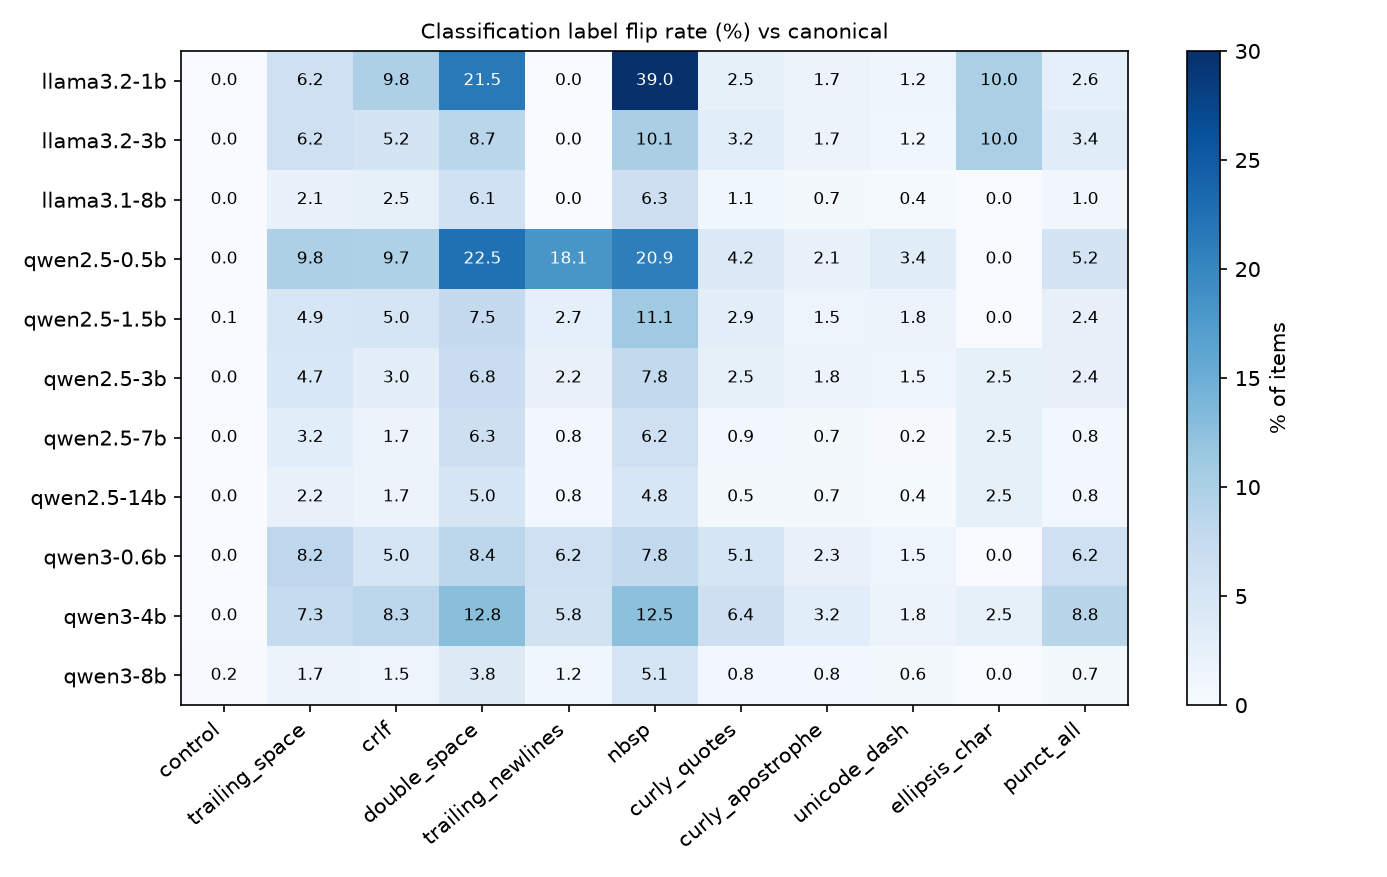
\includegraphics[width=0.85\linewidth]{figures/heat_cls_flip.png}
    \caption{Classification label-flip rate (\%) per model and edit. Llama-3.2-1B under \cond{nbsp} reaches 39\%, and \qwentwo-0.5B under a single trailing \texttt{\textbackslash n\textbackslash n} reaches 18\%. The Llama \cond{trailing_newlines} column is exactly 0 because Llama chat templates strip trailing whitespace, so the model never sees the edit (a placebo). Punctuation columns stay below 1\% for $\geq$7B models.}
    \label{fig:heat}
\end{figure}

\Figref{fig:heat} and \tabref{tab:per_model} show results per model.
Whitespace exceeds punctuation for all 11 models on label flips, code text changes and code pass/fail flips.
Rates span two orders of magnitude, from 0\% (Llama under \cond{trailing_newlines}) to 39\% (Llama-3.2-1B under \cond{nbsp}).
The one exception to the whitespace-first ordering is \qwenthree-8B's raw classification \emph{text}, which changes as often under punctuation as under whitespace. Most of these changes are capitalization of the same label (\texttt{positive} $\rightarrow$ \texttt{Positive}) and do not flip the label.

\begin{table}[t]
    \centering
    \small
    \resizebox{\textwidth}{!}{%
    \begin{tabular}{@{}lcccccccc@{}}
        \toprule
        & & \multicolumn{3}{c}{\textbf{Classification label flip}} & \multicolumn{2}{c}{\textbf{Code (all edits)}} & \multicolumn{2}{c}{\textbf{Control}} \\
        \cmidrule(lr){3-5} \cmidrule(lr){6-7} \cmidrule(lr){8-9}
        \textbf{Model} & \textbf{Params (B)} & Whitespace & Punctuation & All & changed & pass/fail flip & cls flip & code changed \\
        \midrule
        \qwentwo-0.5B & 0.5 & {\bf 16.2} & 3.7 & {\bf 10.6} & 47.8 & 6.3 & 0.0 & 5.2 \\
        \qwenthree-0.6B & 0.6 & 7.1 & 3.8 & 5.6 & 40.4 & 6.0 & 0.0 & 20.9 \\
        Llama-3.2-1B & 1.2 & 15.3 & 2.0 & 9.4 & 29.3 & 3.7 & 0.0 & 15.1 \\
        \qwentwo-1.5B & 1.5 & 6.2 & 2.1 & 4.4 & 38.9 & 6.4 & 0.1 & 3.2 \\
        \midrule
        \qwentwo-3B & 3.1 & 4.9 & 2.0 & 3.6 & 45.1 & {\bf 7.6} & 0.0 & 4.3 \\
        Llama-3.2-3B & 3.2 & 6.1 & 2.4 & 4.4 & 27.3 & 3.8 & 0.0 & 2.2 \\
        \qwenthree-4B & 4.0 & 9.4 & {\bf 5.0} & 7.4 & 28.6 & 3.9 & 0.0 & 0.9 \\
        \qwentwo-7B & 7.6 & 3.6 & 0.7 & 2.3 & 37.3 & 5.7 & 0.0 & 1.9 \\
        Llama-3.1-8B & 8.0 & 3.4 & 0.8 & 2.2 & 29.5 & 4.3 & 0.0 & 2.4 \\
        \qwenthree-8B & 8.2 & 2.6 & 0.7 & 1.8 & 26.5 & 2.9 & 0.2 & 8.0 \\
        \qwentwo-14B & 14.8 & 2.9 & 0.6 & 1.9 & {\bf 49.1} & 6.0 & 0.0 & 7.1 \\
        \bottomrule
    \end{tabular}
    }
    \caption{Divergence (\%) per model. The horizontal rule separates small ($<$3B) from large ($\geq$3B) models. The highest value in each perturbation column is in bold. Whitespace exceeds punctuation for every model. Small models dominate classification flips, while code text changes show no size trend. Control columns show batch-position noise, which is negligible for labels but reaches 21\% of code outputs for \qwenthree-0.6B.}
    \label{tab:per_model}
\end{table}


{\bf Are small models more sensitive?}
\Tabref{tab:size} answers this question.
On classification, models under 3B parameters flip 2.22$\times$ as often as larger models \ci{2.03}{2.41}, and 2.88$\times$ within the \qwentwo family alone.
The GEE model agrees (odds ratio 2.39 for small models, $p<10^{-78}$).
On code, there is no size effect.
Large models change their code text as often as small ones (ratio 0.89 on the excess over control), and pass/fail flips do not differ significantly (1.14, CI includes 1; GEE odds ratio 1.16, $p=0.14$).
\Figref{fig:size} shows that sensitivity is not monotone in size: \qwenthree-4B (7.4\% label flips) is more sensitive than \qwenthree-0.6B (5.6\%).
Part of this is a floor effect.
\qwenthree-0.6B labels 80\% of \agnews items as ``sports'', and Llama-3.2-1B answers ``no'' to 95\% of \boolq items. A near-constant predictor cannot flip.

\begin{table}[t]
    \centering
    \small
    \begin{tabular}{@{}lccc@{}}
        \toprule
        \textbf{Metric} & \textbf{Small ($<$3B)} & \textbf{Large ($\geq$3B)} & \textbf{Ratio small/large} \\
        \midrule
        Classification label flip (all 11 models) & 7.50 & 3.38 & {\bf 2.22} \ci{2.03}{2.41} \\
        Classification label flip (\qwentwo only) & 7.49 & 2.60 & {\bf 2.88} \ci{2.55}{3.32} \\
        Code changed, excess over control & 27.4 & 30.8 & 0.89 \ci{0.84}{0.94} \\
        Code pass/fail flip & 5.51 & 4.83 & 1.14 \ci{0.96}{1.37} \\
        \bottomrule
    \end{tabular}
    \caption{Effect of model size (\%). Ratios use a paired bootstrap over items with 95\% CIs. Small models are 2--3$\times$ more label-sensitive (bold), but they are not more sensitive on code. The \qwentwo-only row compares 0.5B/1.5B with 3B/7B/14B.}
    \label{tab:size}
\end{table}


\begin{figure}[t]
    \centering
    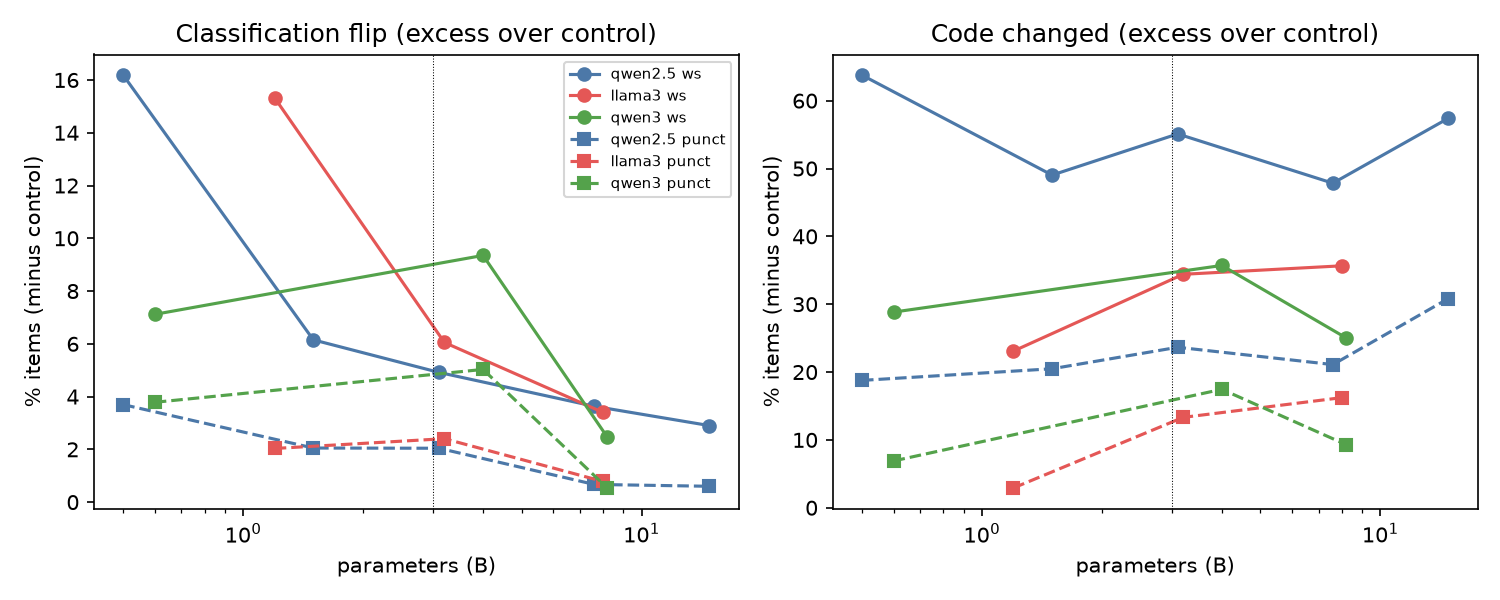
\includegraphics[width=0.9\linewidth]{figures/size_trend.png}
    \caption{Excess divergence over the control \versus parameter count (log scale), per family. Solid lines are whitespace edits, dashed lines punctuation edits, and the dotted vertical line marks 3B. \figleft label flips fall with size for \qwentwo and \llama, while \qwenthree peaks at 4B. \figright code text changes show no downward trend with size. Whitespace lies above punctuation for every family and size.}
    \label{fig:size}
\end{figure}

\subsection{Task type}
\label{sec:res_task}

\Tabref{tab:task} reports divergence per task.
Among classification tasks, flip rates track task ambiguity. The four-way \agnews task, with many borderline Business, Sci/Tech and World items, flips 8.5\% of labels, about three times \sst (3.0\%) and \boolq (3.1\%).
Code text is the most volatile output: 50.3\% of \humaneval and 27.7\% of \mbpp generations change.
Measured by test outcome, however, code is about as affected as classification: 5.1\% of programs change pass/fail status, compared with 4.9\% of labels.
In total, 31\% of perturbed code generations changed their text without changing their test outcome.

\begin{table}[t]
    \centering
    \small
    \begin{tabular}{@{}lccccc@{}}
        \toprule
        & \sst & \boolq & \agnews & \mbpp & \humaneval \\
        \midrule
        Label / pass-fail flip (\%) & 3.0 & 3.1 & {\bf 8.5} & 4.2 & 6.7 \\
        Code changed (\%) & -- & -- & -- & 27.7 & {\bf 50.3} \\
        \bottomrule
    \end{tabular}
    \caption{Divergence per task, averaged over edits and models. The most affected task in each row is in bold. Functional flips are similar across task kinds, while raw code text is far more volatile than labels.}
    \label{tab:task}
\end{table}

\subsection{What drives the effect?}
\label{sec:res_mediators}

\para{The edit must survive the tokenizer.}
When the chat template and tokenizer produce an identical token sequence, outputs change only at the noise-floor rate: 0.02\% label flips and 0.6\% pass/fail flips.
This happens for \cond{trailing_newlines} under Llama templates, which trim trailing whitespace.
When the token sequence changes, flips rise to 5.0\% (classification) and 5.3\% (code pass/fail).
Whether an edit matters therefore depends on the serving template as much as on the model.
The same \texttt{\textbackslash n\textbackslash n} flips 18\% of \qwentwo-0.5B labels and none of Llama's.

\para{Larger edits matter more, but do not explain the gap.}
Divergence grows with the number of changed tokens (odds ratio 1.40 per unit of $\log(1+\Delta\text{tok})$ for label flips).
Adding this term to the GEE model moves the punctuation odds ratio from 0.28 to 0.45 for label flips and from 0.30 to 0.73 for code text changes, but punctuation remains significantly less disruptive.
Matched pairs confirm this.
\cond{trailing_newlines} (\dtok $\approx$ 0.7) flips 3.4\% of labels while \cond{unicode_dash} (\dtok $\approx$ 1.3) flips 1.3\%, and \cond{crlf} (4.3 tokens) flips 4.9\% while \cond{curly_quotes} (6.1 tokens) flips 2.7\%.

\para{Flips land on uncertain items.}
Flips concentrate on items the model gets wrong under the canonical prompt.
For $\geq$7B models, 7.8--9.3\% of wrongly answered items flip, compared with 0.6--1.3\% of correctly answered ones.

\para{Accuracy barely moves.}
Flips are nearly symmetric: 42\% go from right to wrong and 40\% from wrong to right.
The mean accuracy change per model and edit family stays within $\pm$1.3\pp, and most changes are within $\pm$0.7\pp.
The largest drop is Llama-3.2-1B under whitespace edits (2.8\pp \decrease on classification). Whitespace lowers code pass@1 by 0.56\pp on average.
Invisible formatting therefore adds variance to individual predictions rather than a systematic bias.
